\documentclass[conference,twocolumn]{IEEEtran}
\IEEEoverridecommandlockouts
\setlength{\parindent}{2em}
\ifCLASSINFOpdf
\else
\fi
\usepackage{graphicx}
\usepackage{epsfig}
\usepackage{algorithm}
\usepackage{algpseudocode}
\usepackage{amsthm}
\usepackage{subfigure}
\usepackage{float}
\usepackage{amssymb}
\usepackage{caption}
\usepackage{textcomp}
\usepackage{setspace}
\usepackage{xeCJK}
\usepackage{fontspec}
\usepackage{xcolor}
\let\oldemptyset\emptyset
\let\emptyset\varnothing
\usepackage{graphicx}
\usepackage{bm}
\usepackage{enumitem}   
\usepackage{amsmath,amsfonts,amssymb,mathabx,mathtools}
\bibliographystyle{IEEEtran}
\newtheorem{thm}{Theorem}[section]
\newtheorem{cor}[thm]{Corollary}
\newtheorem{lem}[thm]{Lemma}
\newtheorem{cod}[thm]{Condition}
\newtheorem{rmk}{Remark}
\newtheorem{pf}{Proof}
\newtheorem{pot}{Proof of Theorem \ref{thm2}}
\DeclareMathOperator{\Tr}{Tr}
\DeclareMathOperator*{\argmin}{arg\,min}
\theoremstyle{definition}
\newtheorem{definition}{Definition}[section]
\setCJKmainfont{標楷體}  
\XeTeXlinebreaklocale "zh"  
\XeTeXlinebreakskip = 0pt plus 1pt 

\begin{document}
\title{結構化機器學習模型HW1(MLP)}
\author{\IEEEauthorblockN{陳慧如}\\
		    \IEEEauthorblockA{Department of Applied Mathmatics\\
			National Chung Hsing University\\
			South District, Taichung City 40227, Taiwan \\
luluchenyo@smail.nchu.edu.tw}}
	\maketitle	
	\begin{singlespace}
	\IEEEpeerreviewmaketitle
\section{實作項目}
\begin{enumerate}
\item housing data
\item cost function: MSE
\item multi-layer
\item Xavier initialization
\item dropout
\item objective function: R-square
\end{enumerate}

\end{singlespace}
\begin{singlespace}
\section{實作結果}
\begin{enumerate}
\item 3、5、7層
\item default(左)
\item Xavier initialization(中)
\item dropout(右)
\item objective function: R-square(上)
\item cost function: MSE(下)
\end{enumerate}

\subsection{3layers: default VS. Xavier VS. dropout}\ref{f1}

\begin{figure}
\centerline{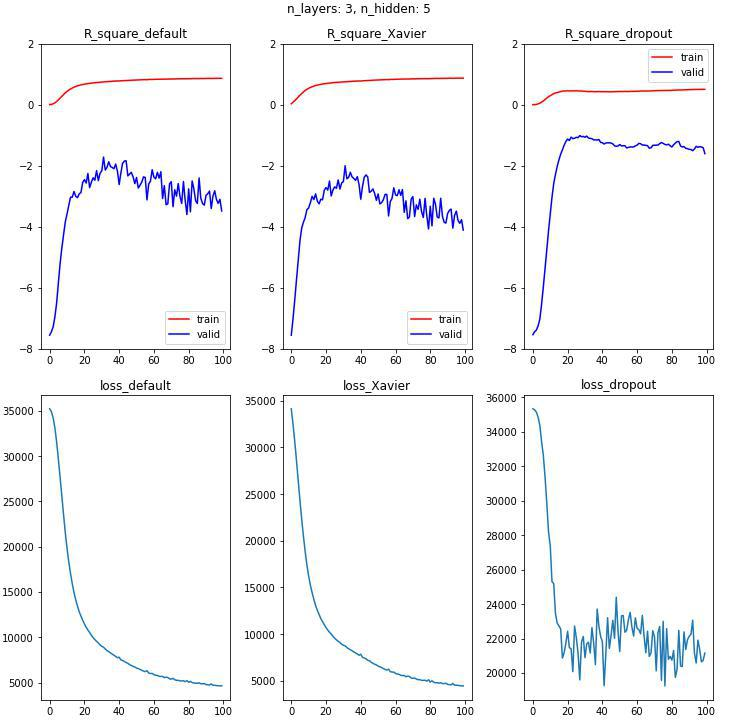
\includegraphics[width=8.5cm, height=10cm]{f1.jpg}}
\caption{3layers: default VS. Xavier VS. dropout}
\label{f1}
\end{figure}
在層數設定為三層的情況下,用dropout的validation R-square分數較高。
\end{singlespace}
\begin{singlespace}

\subsection{5layers: default VS. Xavier VS. dropout}\ref{f2}
\begin{figure}
\centerline{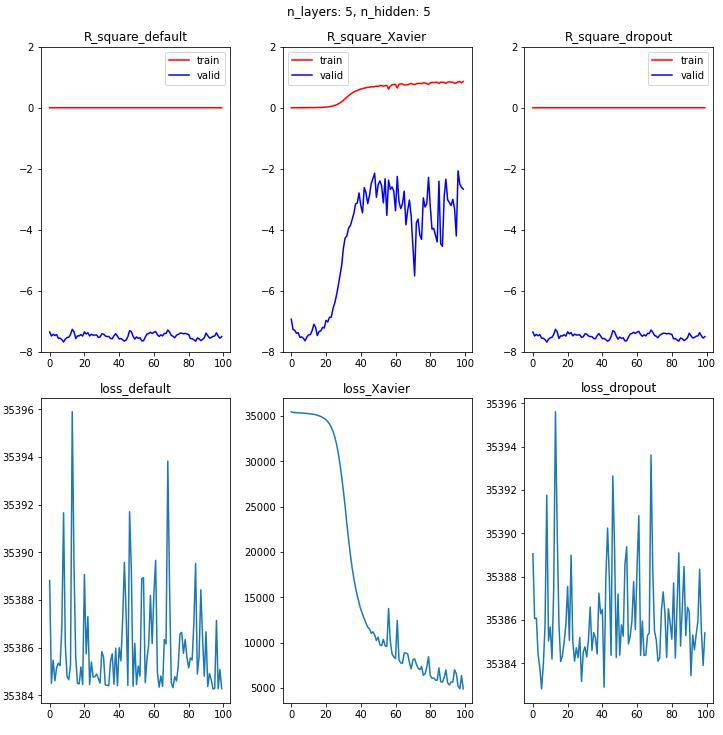
\includegraphics[width=8.5cm, height=10cm]{f2.jpg}}
\caption{5layers: default VS. Xavier VS. dropout}
\label{f2}
\end{figure}
\end{singlespace}
\begin{singlespace}
在層數設定為五層的情況下,用Xavier initializer的結果相對較好。
\end{singlespace}
\begin{singlespace}

\subsection{7layers: default VS. Xavier VS. dropout}\ref{f3}
\begin{figure}
\centerline{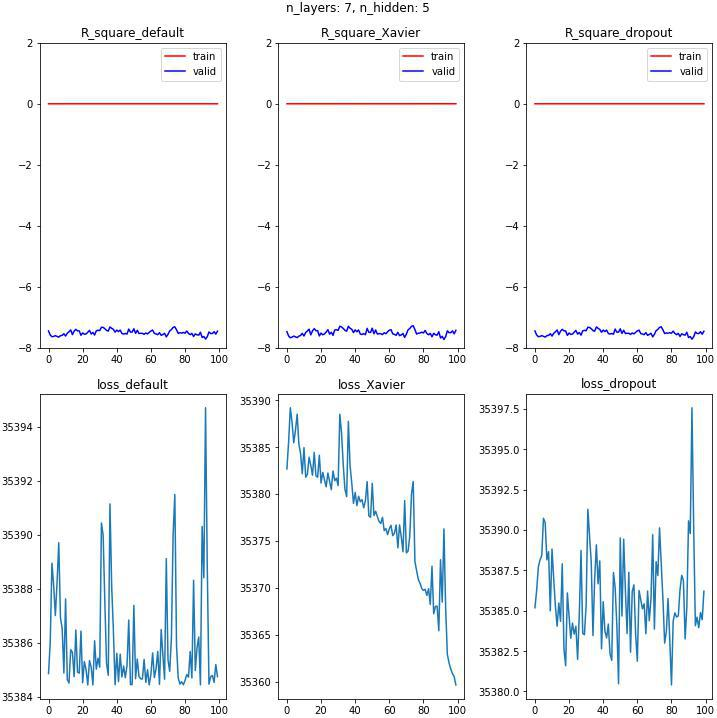
\includegraphics[width=8.5cm, height=10cm]{f3.jpg}}
\caption{7layers: default VS. Xavier VS. dropout}
\label{f3}
\end{figure}
\end{singlespace}
\begin{singlespace}

在層數設定為七層的情況下,只有用Xavier initializer的loss有下降的感覺。
\end{singlespace}
\begin{singlespace}

\end{singlespace}
\begin{singlespace}
\section{結論}
用不同層數、不同初始化參數的方式,試了有dropout跟沒dropout的模型,vilidation的R-square都是負的,雖然loss大部分都有下降,但對於預測房價還是有點困難的。
\end{singlespace}


\end{document}





